% Autogenerated translation of README.md by Texpad
% To stop this file being overwritten during the typeset process, please move or remove this header

\documentclass[12pt]{book}
\usepackage{graphicx}
\usepackage{fontspec}
\usepackage[utf8]{inputenc}
\usepackage[a4paper,left=.5in,right=.5in,top=.3in,bottom=0.3in]{geometry}
\setlength\parindent{0pt}
\setlength{\parskip}{\baselineskip}
\setmainfont{Helvetica Neue}
\usepackage{hyperref}
\pagestyle{plain}
\begin{document}

\chapter*{SkullPos - Software for Kran-o-tron}

Craniofacial Superimposition device over Ethernet between a RPI3 and *nix machine. Interface via command line or graphical interface modes.

This project was completed under the guidance of Carl Stephan of UQ.

\includegraphics{./support/demo2.gif}

\section*{Quick Start}

Uses Python 3 and the TCP/IP stack to communicate with a Raspberry Pi.

Run \texttt{./rasp-install.sh} to enable all requirements on the Raspberry Pi machine. Similarly \texttt{./mach-install.sh} for the client.

Run \texttt{./rasp.sh} on the Raspberry Pi to begin the server process. Note the ipv4 address in the format \texttt{000.000.000.000}.

Run \texttt{./mach.sh $<$addr$>$} on your host machine connected to the Raspberry Pi via Ethernet, where \texttt{$<$addr$>$} is the ipv4 address. This will start the program in GUI mode.

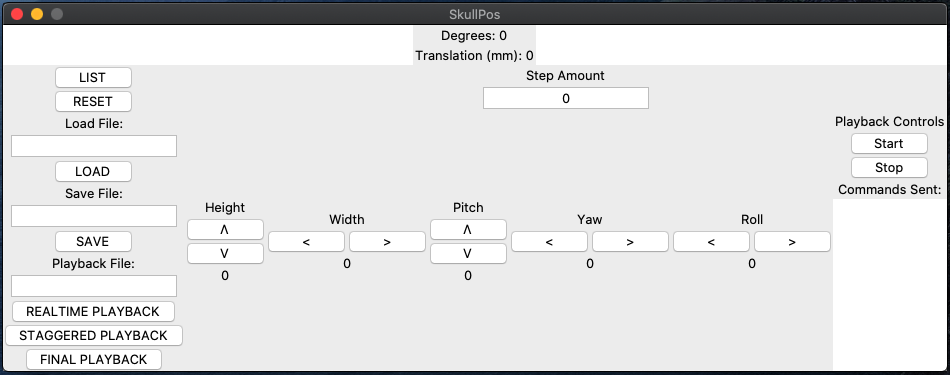
\includegraphics{./support/gui.png}

\section*{Commands}

\subsection*{General}

Use \texttt{pitch}, \texttt{yaw}, \texttt{roll}, \texttt{height} and \texttt{width} like so \texttt{$<$cmd$>$::$<$amount$>$} where \texttt{amount} is the value to operate the servo by.

\texttt{save::$<$name$>$} to save the current position of the device to disk for later use.

\texttt{load::$<$name$>$} to load a profile onto the Pi with the given name from disk.

\texttt{list} to see all current profiles on disk.

\texttt{reset} to reset all positions to their origin.

\texttt{close} to politely close the connection. \texttt{\textasciicircum{}C} also works too.

\subsection*{Playback}

\texttt{playback::START} to begin recording of commands

\texttt{playback::END} to end recording of commands, outputs history to a PDF file.

\texttt{playback::$<$file\_name$>$} to begin playback of a file with a particular name. Must be located in the \texttt{playbacks/} folder.

\texttt{playback::IRL} to set playback mode to perform in \emph{real time} (i.e. playback of commands occurs with the time delay originally performed at).

\texttt{playback::CONTROL} to set playback mode to perform the next command with input from the user (i.e. hitting any key).

\texttt{playback\_final::$<$file\_name$>$} jump straight to the final position of a Kran-o-tron session file. Must be located in the \texttt{playbacks/} folder.

By default, on starting the software, all commands sent across to Kran-o-tron are recorded in a file with the date and time that Kran-o-tron was accessed for that session. This is found in the \texttt{playback/} directory.

To turn this off, use the flag \texttt{-no\_playback} when starting \texttt{./mach.sh}.

See above for a list of commands to control playback.

\section*{Profile format}

All position profiles are stored in \texttt{profiles.json} in the home directory for easy to edit formatting. See the file for formatting examples.

\section*{Miscellaneous}

If GUI mode is undesirable, run \texttt{python3 mach.py $<$addr$>$} to communicate with the Raspberry Pi, where \texttt{$<$addr$>$} is the ipv4 address given above. This will connect to the Pi over ethernet in \emph{command line mode}, thus you will have to issue commands (specified in \href{##Commands}{Commands}).

\section*{Contributors}

\texttt{m-ish} - Hamish Bultitude

\end{document}
